\documentclass[12pt]{scrartcl}

\usepackage[T1]{fontenc}
\usepackage[utf8]{inputenc}
\usepackage{amsmath}
\usepackage{amsfonts}
\usepackage{amssymb}
\usepackage{amsbsy}
\usepackage{graphicx}
\usepackage{float}
\usepackage{array}
\usepackage{booktabs}
\usepackage{multirow}
\usepackage{bm}
\usepackage{verbatim}
\usepackage[english]{babel}
\usepackage{color}
\usepackage{url}
\usepackage{fancybox}
\usepackage[stable]{footmisc}
\usepackage[format=plain,labelfont=bf]{caption}
\usepackage{fancyhdr}
\usepackage{natbib}
\usepackage{calc}
\usepackage{textcomp}
\usepackage[pdftex,pdfborder={0 0 0}]{hyperref}
\usepackage{pdfpages}
\usepackage{tikz}
\usetikzlibrary{shapes,backgrounds,fit,shadows,arrows,positioning}
\usepackage{mathtools}
\usepackage{algorithm}
\usepackage{algorithmic}
\usepackage{placeins}
\usepackage{pifont}
\usepackage{adjustbox}

% Define the layers to draw the diagram
\pgfdeclarelayer{background}
\pgfdeclarelayer{foreground}
\pgfsetlayers{background,main,foreground}
\pagenumbering{gobble}

% Define block styles
\tikzstyle{process} = [draw, fill=blue!20, text centered, text width=13em, minimum width=8em, minimum height=3em, rounded corners, drop shadow,font=\bfseries]
\tikzstyle{inputdata} = [draw, fill=green!20, text centered, text width=6em, minimum width=3em, minimum height=3em, drop shadow,font=\bfseries]
\tikzstyle{tmpdata} = [draw, fill=orange!20, text centered, text width=6em, minimum width=3em, minimum height=3em, drop shadow,font=\bfseries]
\tikzstyle{outputdata} = [draw, fill=red!20, text centered, text width=6em, minimum width=3em, minimum height=3em, drop shadow,font=\bfseries]
\tikzstyle{indexdata} = [draw, fill=white, text centered, text width=6em, minimum width=2em, minimum height=2em, rounded corners, font=\bfseries]
\tikzstyle{arrow} = [draw, ultra thick, color=black!50, -latex']
\tikzstyle{line} = [draw, ultra thick, color=black!50]
\tikzstyle{dash} = [dotted, draw, ultra thick, color=black!50, -latex']

% Define distances for bordering
\newcommand{\blockdist}{1.3}
\newcommand{\edgedist}{1.5}
\newcommand{\inputdata}[2]{node (i#1) [inputdata] {#2}}
\newcommand{\tmpdata}[2]{node (t#1) [tmpdata] {#2}}
\newcommand{\outputdata}[2]{node (o#1) [outputdata] {#2}}
\newcommand{\indexdata}[2]{node (d#1) [indexdata] {#2}}
\newcommand{\process}[2]{node (p#1) [process] {#2}}
\newcommand{\background}{%
\begin{pgfonlayer}{background}
\path (d4)+(-2,-1.1) node (a1) {};
\path (d5)+(1.6,1.1) node (a2) {};
\path[fill=yellow!20,rounded corners, draw=black!50, dashed] (a1) rectangle (a2);
\end{pgfonlayer}}

\renewcommand*{\familydefault}{\sfdefault}

% Margins
\addtolength{\textheight}{1.0cm}
\addtolength{\oddsidemargin}{-0.5cm}
\addtolength{\evensidemargin}{-0.5cm}
\addtolength{\textwidth}{1.0cm}
\parindent=0em

% Appropriate font for \mathcal{}
\DeclareSymbolFont{cmmathcal}{OMS}{cmsy}{m}{n}
\DeclareSymbolFontAlphabet{\mathcal}{cmmathcal}

% Set subscript and superscripts positions
\everymath{
\fontdimen13\textfont2=5pt
\fontdimen14\textfont2=5pt
\fontdimen15\textfont2=5pt
\fontdimen16\textfont2=5pt
\fontdimen17\textfont2=5pt
}

% Bibliography style
\setlength{\bibsep}{1pt}

% Part
\renewcommand\partheadstartvskip{\clearpage\null\vfil}
\renewcommand\partheadmidvskip{\par\nobreak\vskip 20pt\thispagestyle{empty}}
\renewcommand\partheadendvskip{\vfil\clearpage}
\renewcommand\raggedpart{\centering}

 % Checkmark
\newcommand{\cmark}{\ding{51}}%
\newcommand{\xmark}{\ding{55}}%

\begin{document}

\title{\vspace{-1.2cm}Guess consistency for\\
multi-incremental minimization}
\author{Benjamin Ménétrier}
\date{Last update: \today\vspace{-0.5cm}}

\thispagestyle{empty}

\maketitle

\tableofcontents

\section{Problem linearization}

\subsection{Full cost function}
The full cost function to minimize is defined as:
\begin{align}
\hspace{-0.7cm} \mathcal{J}(\mathbf{x}) = \frac{1}{2} \left(\mathbf{x}-\mathbf{x}^b\right)^\mathrm{T} \mathbf{B}^{-1} \left(\mathbf{x}-\mathbf{x}^b\right) + \frac{1}{2} \left(\mathbf{y}^o-\mathcal{H}(\mathbf{x})\right)^\mathrm{T} \mathbf{R}^{-1} \left(\mathbf{y}^o-\mathcal{H}(\mathbf{x})\right)
\end{align}
where:
\begin{itemize}
\item $\mathbf{x} \in \mathbb{R}^n$ is the state in model space,
\item $\mathbf{x}^b \in \mathbb{R}^n$ is the background state,
\item $\mathbf{R} \in \mathbb{B}^{n \times n}$ is the background error covariance matrix,
\item $\mathbf{y}^o \in \mathbb{R}^p$ is the observation vector,
\item $\mathbf{R} \in \mathbb{R}^{p \times p}$ is the observation error covariance matrix,
\item $\mathcal{H} : \mathbb{R}^n \rightarrow \mathbb{R}^p$ is the nonlinear observation operator.
\end{itemize}

\subsection{Quadratic cost function}
Instead of minimizing the full cost function $\mathcal{J}(\mathbf{x})$, we minimize successive quadratic approximations around a guess state $\mathbf{x}^g_k$, for $k \in [1,K]$. The increment $\delta \mathbf{x}_k \in \mathbb{R}^n$ is defined as:
\begin{align}
\delta \mathbf{x}_k =  \mathbf{x}-\mathbf{x}^g_k
\end{align}
and is used to linearize the observation operator for $\mathbf{x} \approx \mathbf{x}^g_k$:
\begin{align}
\label{eq:linearize}
\mathcal{H}(\mathbf{x}) & \approx \mathcal{H}(\mathbf{x}^g_k) + \mathbf{H}_k \delta \mathbf{x}_k
\end{align}
where $\mathbf{H}_k \in \mathbb{R}^{p \times n}$ is the observation operator linearized around $\mathbf{x}^g_k$:
\begin{align}
\label{eq:h_linearization}
H_{k,ij} = \left.\frac{\partial \mathcal{H}_i}{\partial x_j}\right|_{\mathbf{x} = \mathbf{x}^g_k}
\end{align}
Thus, the quadratic cost function is given by:
\begin{align}
\label{eq:cost_quad}
J \left(\delta \mathbf{x}_k\right) = \frac{1}{2} \left(\delta \mathbf{x}_k-\delta \mathbf{x}^b_k\right)^\mathrm{T} \mathbf{B}^{-1} \left(\delta \mathbf{x}_k-\delta \mathbf{x}^b_k\right) + \frac{1}{2} \left(\mathbf{d}_k - \mathbf{H}_k \delta \mathbf{x}_k\right)^\mathrm{T} \mathbf{R}^{-1} \left(\mathbf{d}_k - \mathbf{H}_k \delta \mathbf{x}_k\right)
\end{align}
where:
\begin{itemize}
\item $\delta \mathbf{x}^b_k  \in \mathbb{R}^n$ is the background increment:
\begin{align}
\delta \mathbf{x}^b_k = \mathbf{x}^b - \mathbf{x}^g_k
\end{align}
\item $\mathbf{d}_k \in \mathbb{R}^p$ is the innovation vector:
\begin{align}
\label{eq:innovation}
\mathbf{d}_k = \mathbf{y}^o - \mathcal{H}(\mathbf{x}^g_k)
\end{align}
\end{itemize}
The minimization of each quadratic approximation is called ``outer iteration'', and should be distinguished from the ``inner iterations'' required in classical algorithms (conjugate gradient, Lanczos method) to find the minimum of a quadratic approximation.

\subsection{Linear system}
Setting the gradient of $J(\delta \mathbf{x}_k)$ to zero gives the analysis increment $\delta \mathbf{x}^a_k$:
\begin{align}
\label{eq:inc}
& \ \mathbf{B}^{-1} \left(\delta \mathbf{x}^a_k - \delta \mathbf{x}^b_k\right) - \mathbf{H}_k^\mathrm{T} \mathbf{R}^{-1} \left(\mathbf{d}_k - \mathbf{H}_k \delta \mathbf{x}^a_k\right) = 0 \nonumber \\
\Leftrightarrow & \ \left(\mathbf{B}^{-1} + \mathbf{H}_k^\mathrm{T} \mathbf{R}^{-1} \mathbf{H}_k\right) \delta \mathbf{x}^a_k = \mathbf{B}^{-1} \delta \mathbf{x}^b_k + \mathbf{H}_k^\mathrm{T} \mathbf{R}^{-1} \mathbf{d}_k \nonumber \\
\Leftrightarrow & \ \boxed{\mathbf{A}^\mathbf{x}_k \delta \mathbf{x}^a_k = \mathbf{b}^\mathbf{x}_k}
\end{align}
with $\mathbf{A}^\mathbf{x}_k \in \mathbb{R}^{n \times n}$ and $\mathbf{b}^\mathbf{x}_k \in \mathbb{R}^{n}$ defined as:
\begin{align}
\mathbf{A}^\mathbf{x}_k & = \mathbf{B}^{-1} + \mathbf{H}_k^\mathrm{T} \mathbf{R}^{-1} \mathbf{H}_k \\
\mathbf{b}^\mathbf{x}_k & = \mathbf{B}^{-1} \delta \mathbf{x}^b_k + \mathbf{H}_k^\mathrm{T} \mathbf{R}^{-1} \mathbf{d}_k
\end{align}

\subsection{Square-root $\mathbf{B}$ preconditioning}
Since $\mathbf{B}$ is positive definite, there is an infinity of square-roots $\mathbf{U} \in \mathbb{R}^{n \times m}$ with $m \ge n$ verifying:
\begin{align}
\mathbf{B} = \mathbf{U} \mathbf{U}^\mathrm{T}
\end{align}

\subsubsection{Classic variable change}
A new variable $\delta \mathbf{v}_k \in \mathbb{R}^m$ is defined as:
\begin{align}
\label{eq:deltav}
\delta \mathbf{v}_k = \mathbf{U}^\mathrm{T} \mathbf{B}^{-1} \delta \mathbf{x}_k
\end{align}
leading to
\begin{align}
\label{eq:deltax_to_deltav}
\boxed{\delta \mathbf{x}_k = \mathbf{U} \delta \mathbf{v}_k}
\end{align}
Using variable change \eqref{eq:deltax_to_deltav} and applying $\mathbf{U}^\mathrm{T}$ on both sides, the linear system \eqref{eq:inc} can be transformed into:
\begin{align}
\label{eq:inc_U}
\boxed{\mathbf{A}^\mathbf{v}_k \delta \mathbf{v}^a_k = \mathbf{b}^\mathbf{v}_k}
\end{align}
with $\mathbf{A}^\mathbf{v}_k \in \mathbb{R}^{m \times m}$ and $\mathbf{b}^\mathbf{v}_k \in \mathbb{R}^{m}$ defined as:
\begin{align}
\mathbf{A}^\mathbf{v}_k & = \mathbf{I}_m + \mathbf{U}^\mathrm{T} \mathbf{H}_k^\mathrm{T} \mathbf{R}^{-1} \mathbf{H}_k \mathbf{U} \\
\mathbf{b}^\mathbf{v}_k & = \delta \mathbf{v}^b_k + \mathbf{U}^\mathrm{T} \mathbf{H}_k^\mathrm{T} \mathbf{R}^{-1} \mathbf{d}_k
\end{align}
with
\begin{align}
\delta \mathbf{v}^b_k = \mathbf{U}^\mathrm{T} \mathbf{B}^{-1} \delta \mathbf{x}^b_k
\end{align}

\subsubsection{Non-classic variable change}
Another new variable $\delta \mathbf{w}_k \in \mathbb{R}^m$ can be defined as:
\begin{align}
\delta \mathbf{w}_k & = \mathbf{U}^\mathrm{T} \mathbf{B}^{-1} \left(\mathbf{x}_k - \mathbf{x}^b\right) \nonumber \\
 & = \mathbf{U}^\mathrm{T} \mathbf{B}^{-1} \left(\delta \mathbf{x}_k - \delta \mathbf{x}^b_k\right)
\end{align}
leading to
\begin{align}
\label{eq:deltax_to_deltaw}
\boxed{\delta \mathbf{x}_k = \mathbf{U} \delta \mathbf{w}_k + \delta \mathbf{x}^b_k}
\end{align}
The link between $\delta \mathbf{w}_k$ and $\delta \mathbf{v}_k$ is straightforward:
\begin{align}
\label{eq:link_deltaw-deltav}
\delta \mathbf{v}_k = \delta \mathbf{w}_k + \delta \mathbf{v}^b_k
\end{align}
Using variable change \eqref{eq:deltax_to_deltaw} and applying $\mathbf{U}^\mathrm{T}$ on both sides, the linear system \eqref{eq:inc} can be transformed into:
\begin{align}
\label{eq:inc_U_w}
\boxed{\mathbf{A}^\mathbf{v}_k \delta \mathbf{w}^a_k = \mathbf{b}^\mathbf{w}_k}
\end{align}
with $\mathbf{b}^\mathbf{w}_k \in \mathbb{R}^{m}$ defined as:
\begin{align}
\mathbf{b}^\mathbf{w}_k & = \mathbf{U}^\mathrm{T} \mathbf{H}_k^\mathrm{T} \mathbf{R}^{-1} \left(\mathbf{d}_k - \mathbf{H}_k \delta \mathbf{x}^b_k\right)
\end{align}
The obvious advantage of this second option is to get rid of $\mathbf{B}^{-1}$ in the right-hand side $\mathbf{b}^\mathbf{w}_k$, whereas it is required in the right-hand side $\mathbf{b}^\mathbf{v}_k$ for the term $\delta \mathbf{v}^b_k$.

\subsection{Minimizer starting state}
A starting state $\mathbf{x}^s_k$ has to be defined for each outer iteration, and converted into control space:
\begin{itemize}
\item For the classic variable change, the starting increment in control space is:
\begin{align}
\delta \mathbf{v}^s_k = \mathbf{U}^\mathrm{T} \mathbf{B}^{-1} \left(\mathbf{x}^s_k-\mathbf{x}^g_k\right)
\end{align}
\item For the non-classic variable change, the starting increment in control space is:
\begin{align}
\delta \mathbf{w}^s_k = \mathbf{U}^\mathrm{T} \mathbf{B}^{-1} \left(\mathbf{x}^s_k-\mathbf{x}^b\right)
\end{align}
\end{itemize}
The most obvious choice for the starting state $\mathbf{x}^s_k$ is the guess $\mathbf{x}^g_k$, since it is the best estimate of the final analysis we have at a given outer iteration. In this case:
\begin{itemize}
\item For the classic variable change:
\begin{align}
\delta \mathbf{v}^s_k = 0
\end{align}
\item For the non-classic variable change:
\begin{align}
\delta \mathbf{w}^s_k & = -\mathbf{U}^\mathrm{T} \mathbf{B}^{-1} \delta \mathbf{x}^b_k \nonumber \\
& = - \delta \mathbf{v}^b_k
\end{align}
It should be noted that $\mathbf{B}^{-1}$ is absent from the right-hand side $\mathbf{b}^\mathbf{w}_k$ but it is required in the starting increment $\delta \mathbf{w}^s_k$.
\end{itemize}
Another possible starting state $\mathbf{x}^s_k$ for the non-classic variable change is the background $\mathbf{x}^b$, leading to a starting increment $\delta \mathbf{w}^s_k = 0$. This option removes the need for $\mathbf{B}^{-1}$ completely, but is not explored further in this document.

\section{Practical computations}

\subsection{Getting rid of $\mathbf{B}^{-1}$}
In practice, the inverse of the background error covariance matrix $\mathbf{B}^{-1}$ is not available, even if it is needed in general to compute the background increment $\delta \mathbf{v}^b_k$, required for the right-hand side $\mathbf{b}^\mathbf{v}_k$ or for the starting increment $\delta \mathbf{w}^s_k$. However, the analysis is defined as:
\begin{align}
\mathbf{x}^a_k = \mathbf{x}^g_k + \delta \mathbf{x}^a_k
\end{align}
and it seems logical to define the guess as the analysis of the previous outer iteration:
\begin{itemize}
\item for $k = 1$: $\mathbf{x}^g_1 = \mathbf{x}^b$,
\item for $k > 1$: $\mathbf{x}^g_k = \mathbf{x}^a_{k-1}$.
\end{itemize}
Thus:
\begin{itemize}
\item for $k = 1$:
\begin{align}
\delta \mathbf{x}^b_1 = \mathbf{x}^g_1 - \mathbf{x}^b = 0
\end{align}
\item for $k > 1$:
\begin{align}
\delta \mathbf{x}^b_k & = \mathbf{x}^b - \mathbf{x}^g_k \nonumber \\
& = \mathbf{x}^b - \mathbf{x}^a_{k-1} \nonumber \\
& = \mathbf{x}^b - \left(\mathbf{x}^g_{k-1} + \delta \mathbf{x}^a_{k-1}\right) \nonumber \\
& = \delta \mathbf{x}^b_{k-1} - \delta \mathbf{x}^a_{k-1}
\end{align}
\end{itemize}
which can be combined recursively to yield:
\begin{align}
\label{eq:back_inc}
\delta \mathbf{x}^b_k & = - \sum_{i=1}^{k-1} \delta \mathbf{x}^a_i
\end{align}
Using equation \eqref{eq:deltav} and applying $\mathbf{U}^\mathrm{T} \mathbf{B}^{-1}$ on both sides of equation \eqref{eq:back_inc}, we get:
\begin{align}
\label{eq:back_inc_U}
\boxed{\delta \mathbf{v}^b_k = - \sum_{i=1}^{k-1} \delta \mathbf{v}^a_i}
\end{align}
Using equation \eqref{eq:link_deltaw-deltav}, we get also:
\begin{align}
\delta \mathbf{v}^b_k = - \sum_{i=1}^{k-1} \left(\delta \mathbf{w}^a_i +\delta \mathbf{v}^b_i\right)
\end{align}
So for $k>1$:
\begin{align}
\delta \mathbf{v}^b_k & = - \left(\delta \mathbf{w}^a_{k-1} + \delta \mathbf{v}^b_{k-1} + \sum_{i=1}^{k-2} \left(\delta \mathbf{w}^a_i + \delta \mathbf{v}^b_i\right)\right) \nonumber \\
& = - \left(\delta \mathbf{w}^a_{k-1} + \delta \mathbf{v}^b_{k-1} - \delta \mathbf{v}^b_{k-1}\right)
\end{align}
leading to:
\begin{align}
\label{eq:back_inc_U_w}
\boxed{\delta \mathbf{v}^b_k = - \delta \mathbf{w}^a_{k-1}}
\end{align}

Equation \eqref{eq:back_inc_U} and \eqref{eq:back_inc_U_w} can be used to compute $\mathbf{b}^\mathbf{v}_k$ and $\delta \mathbf{w}^s_k$ respectively, without requiring $\mathbf{B}^{-1}$.

\subsection{Changing the resolution}
For computational efficiency, it is common to start the outer iterations at a lower grid resolution, and to increase it at each outer iteration $k$. At resolution $\mathcal{R}_k$, the model space size is denoted $n_k$ and the control space size $m_k$. It is assumed hereafter that:
\begin{itemize}
\item resolutions are stricly increasing: for $i < k$, $n_i < n_k$ and $m_i < m_k$,
\item the full resolution is obtained at the last iteration $K$.
\end{itemize}
Obviously in this case, $\mathbf{B}$ also depends on iteration $k$. Hereafter, it is denoted $\mathbf{B}_k$, and its square-root is denoted $\mathbf{U}_k$. The previous trick to get rid of $\mathbf{B}^{-1}$ no longer works, since the control vector size changes at each outer iteration.

\subsection{Interpolators}
We define two linear interpolators from resolution $\mathcal{R}_i$ to resolution $\mathcal{R}_k$:
\begin{itemize}
\item $\mathbf{T}^\mathbf{x}_{i \rightarrow k} \in \mathbb{R}^{n_k \times n_i}$ in model space,
\item $\mathbf{T}^\mathbf{v}_{i \rightarrow k} \in \mathbb{R}^{m_k \times m_i}$ in control space,
\end{itemize}
$  $\\
Interpolators can be applied on ``states'' (i.e. physical quantities) like the background or the guess, or on ``increments'' (i.e. differences of physical quantities), which are denoted with a $\delta$ in this document. For downscaling, it seems reasonable to apply interpolators on either states or increments. However for upscaling, it seems better to apply interpolators on increments only and to add these increments to high resolution states, rather than to upscale states directly. Indeed, high resolution states already have meaningful small scale features, whereas upscaled states do not.

\subsection{Analysis at high resolution}
As a consequence, the multi-resolution problem should be solved with the following requirements in mind:
\begin{itemize}
\item The background $\mathbf{x}^b$ is provided at full resolution, but it can be simplified at resolution $\mathcal{R}_k$:
\begin{align}
\boxed{\mathbf{x}^b_k = \mathbf{T}^\mathbf{x}_{K \rightarrow k} \mathbf{x}^b}
\end{align}
\item A full resolution guess denoted $\mathbf{x}^{g+}_k$ has to be computed at each outer iteration to run model trajectories used in the operators linearization. This full resolution guess can be simplified at resolution $\mathcal{R}_k$ to give the actual guess of outer iteration $k$:
\begin{align}
\boxed{\mathbf{x}^g_k = \mathbf{T}^\mathbf{x}_{K \rightarrow k} \mathbf{x}^{g+}_k}
\end{align}
\item Only increments should be interpolated to higher resolution, and then possibly added to states at high resolution.
\end{itemize}

At each outer iteration, the analysis increment $\delta \mathbf{x}^a_k$ is given at resolution $\mathcal{R}_k$ for the classic variable change by:
\begin{align}
\label{eq:analysis_increment}
\delta \mathbf{x}^a_k = \mathbf{U}_k \delta \mathbf{v}^a_k
\end{align}
or for the non-classic variable change by:
\begin{align}
\label{eq:analysis_increment_w}
\delta \mathbf{x}^a_k = \mathbf{U}_k \delta \mathbf{w}^a_k + \delta \mathbf{x}^b_k
\end{align}
and it can be interpolated at full resolution:
\begin{align}
\label{eq:full_res_analysis_increment}
\delta \mathbf{x}^{a+}_k = \mathbf{T}^\mathbf{x}_{k \rightarrow K} \delta \mathbf{x}^a_k
\end{align}
to give the full resolution analysis:
\begin{align}
\label{eq:full_res_analysis}
\mathbf{x}^{a+}_k = \mathbf{x}^{g+}_k+\delta \mathbf{x}^{a+}_k
\end{align}

\section{Guess consistency}

\subsection{Problem clarification}
In the linear system solved at each outer iteration, the full resolution guess $\mathbf{x}^{g+}_k$ appears for two distinct purposes.
\begin{enumerate}
\item It is used explicitly as the linearization state for the nonlinear observation operator in equation \eqref{eq:h_linearization}, and also to compute the innovation $\mathbf{d}_k$ in equation \eqref{eq:innovation}.
\item It is needed implicitly in the background increment $\delta \mathbf{v}^b_k$, required for the right-hand side $\mathbf{b}^\mathbf{v}_k$ or for the starting increment $\delta \mathbf{w}^s_k$:
\begin{align}
\label{eq:correct_dvb}
\delta \mathbf{v}^b_k & = \mathbf{U}_k^\mathrm{T} \mathbf{B}^{-1}_k \delta \mathbf{x}^b_k \nonumber \\
& = \mathbf{U}_k^\mathrm{T} \mathbf{B}^{-1}_k \left(\mathbf{x}^b_k - \mathbf{x}^g_k\right)  \nonumber \\
& = \mathbf{U}_k^\mathrm{T} \mathbf{B}^{-1}_k \mathbf{T}^\mathbf{x}_{K \rightarrow k} \left(\mathbf{x}^b - \mathbf{x}^{g+}_k\right)
\end{align}
\end{enumerate}
For the first outer iteration, the full resolution guess is always taken as the background state (also provided at full resolution):
\begin{align}
\label{eq:usual_full_res_first}
\mathbf{x}^{g+}_1 = \mathbf{x}^b
\end{align}
and the background increment is zero, which is consistent. The goal of this section is to define the possible strategies to maintain this consistency between the two purposes of the high resolution guess in subsequent outer iterations.

\subsection{Theoretical method}
In the theoretical method, $\mathbf{B}_k^{-1}$ is supposed to be available and can be used to compute $\delta \mathbf{v}^b_k$ explicitly from $\mathbf{x}^{g+}_k$ using equation \eqref{eq:correct_dvb}, so the guess consistency is always maintained.\\
$  $\\
For outer iterations $k>1$, the full resolution guess is simply taken as the previous analysis at full resolution:
\begin{align}
\label{eq:usual_full_res}
\mathbf{x}^{g+}_k = \mathbf{x}^{a+}_{k-1}
\end{align}

\subsection{Practical methods}

\subsubsection{Approximations}
In practical methods, $\mathbf{B}_k^{-1}$ is not available and the background increment $\delta \mathbf{v}^b_k$ is computed separately, using an updated version of equation \eqref{eq:back_inc_U} with appropriate interpolations:
\begin{itemize}
\item For the classic variable change:
\begin{align}
\label{eq:back_inc_Uvar}
\boxed{\delta \mathbf{v}^b_k = - \sum_{i=1}^{k-1} \mathbf{T}^\mathbf{v}_{i \rightarrow k} \delta \mathbf{v}^a_i}
\end{align}
\item For the non-classic variable change:
\begin{align}
\label{eq:back_inc_Uvar_w}
\boxed{\delta \mathbf{v}^b_k = - \mathbf{T}^\mathbf{v}_{k-1 \rightarrow k} \delta \mathbf{w}^a_{k-1}}
\end{align}
\end{itemize}

\subsubsection{Consistent method}
In the consistent method, the background increment $\delta \mathbf{v}^b_k$ is obtained from equation \eqref{eq:back_inc_Uvar} or equation \eqref{eq:back_inc_Uvar_w}. From this, the background increment $\delta \mathbf{x}^b_k$ is given by:
\begin{align}
\label{eq:consistent_U}
\delta \mathbf{x}^b_k & = \mathbf{U}_k \delta \mathbf{v}^b_k
\end{align}
It is then interpolated at full resolution:
\begin{align}
\label{eq:full_res_consistent_U}
\delta \mathbf{x}^{b+}_k = \mathbf{T}^\mathbf{x}_{k \rightarrow K} \delta \mathbf{x}^b_k
\end{align}
and the guess at full resolution is deduced as:
\begin{align}
\label{eq:full_res_consistent_guess}
\mathbf{x}^{g+}_k = \mathbf{x}^b - \delta \mathbf{x}^{b+}_k
\end{align}
In this method, the guess at full resolution \textbf{is not equal} to the analysis at full resolution of the previous outer iteration, but the guess consistency is always maintained by construction.

\subsubsection{Standard method}
In the standard method, the full resolution guess is explicitly computed from the analysis of the previous outer iteration. However, contrary to the theoretical method, a correction has to be applied in order to maintain the guess consistency. This correction is neglected in operational data assimilation systems, and the goal of this section is to compute it explicitly.\\
$  $\\
For outer iterations $k>1$, the full resolution guess is now given by:
\begin{align}
\label{eq:usual_full_res_next}
\mathbf{x}^{g+}_k = \mathbf{x}^{a+}_{k-1} + \delta \mathbf{x}^{c+}_{k}
\end{align}
where $\delta \mathbf{x}^{c+}_{k}$ is the correction. Merging equations \eqref{eq:full_res_analysis}, \eqref{eq:usual_full_res_first} and \eqref{eq:usual_full_res_next}, the guess at full resolution can be expressed from the previous iteration:
\begin{align}
\mathbf{x}^{g+}_k & = \mathbf{x}^{a+}_{k-1}+\delta \mathbf{x}^{c+}_k \nonumber \\
& = \mathbf{x}^{g+}_{k-1} + \delta \mathbf{x}^{a+}_{k-1} + \delta \mathbf{x}^{c+}_k \nonumber \\
\end{align}
and recursively backward to the first outer iteration:
\begin{align}
\label{eq:usual_full_res}
\mathbf{x}^{g+}_k = \mathbf{x}^{b} + \sum_{i=1}^{k-1} \delta \mathbf{x}^{a+}_i + \sum_{i=2}^k \delta \mathbf{x}^{c+}_i
\end{align}
Thus, the background increment is given by:
\begin{align}
\delta \mathbf{x}^b_k & = \mathbf{x}^b_k - \mathbf{x}^g_k \nonumber \\
& = \mathbf{T}^\mathbf{x}_{K \rightarrow k} \left(\mathbf{x}^b - \mathbf{x}^{g+}_k\right) \nonumber \\
& = - \mathbf{T}^\mathbf{x}_{K \rightarrow k} \left(\sum_{i=1}^{k-1} \delta \mathbf{x}^{a+}_i + \sum_{i=2}^k \delta \mathbf{x}^{c+}_i\right) \nonumber \\
& = - \left[\mathbf{T}^\mathbf{x}_{K \rightarrow k} \left(\sum_{i=1}^{k-1} \delta \mathbf{x}^{a+}_i + \sum_{i=2}^{k-1} \delta \mathbf{x}^{c+}_i\right) + \mathbf{T}^\mathbf{x}_{K \rightarrow k} \delta \mathbf{x}^{c+}_k\right]
\end{align}
which is equivalent to:
\begin{align}
\mathbf{T}^\mathbf{x}_{K \rightarrow k} \delta \mathbf{x}^{c+}_k = - \left[\mathbf{T}^\mathbf{x}_{K \rightarrow k} \left(\sum_{i=1}^{k-1} \delta \mathbf{x}^{a+}_i + \sum_{i=2}^{k-1} \delta \mathbf{x}^{c+}_i\right) + \delta \mathbf{x}^b_k\right]
\end{align}
In the general case, it is not possible to compute the correction $\delta \mathbf{x}^{c+}_k$ explicitly.

\subsubsection{Special case of transitive interpolators}
A special class of interpolators called ``transitive interpolators'' has three extra properties:
\begin{itemize}
\item Upscaling transitivity: for $n_i < n_j$ and $n_i < n_k$:
\begin{align}
\mathbf{T}^\mathbf{x}_{j \rightarrow k} \mathbf{T}^\mathbf{x}_{i \rightarrow j} = \mathbf{T}^\mathbf{x}_{i \rightarrow k}
\end{align}
\item Downscaling transitivity: for $n_i < n_j < n_k$:
\begin{align}
\mathbf{T}^\mathbf{x}_{j \rightarrow i} \mathbf{T}^\mathbf{x}_{k \rightarrow j} = \mathbf{T}^\mathbf{x}_{k \rightarrow i}
\end{align}
\item Known right-inverse: for $n_i < n_k$
\begin{align}
\mathbf{T}^\mathbf{x}_{k \rightarrow i} \mathbf{T}^\mathbf{x}_{i \rightarrow k} = \mathbf{I}_{n_i}
\end{align}
\end{itemize}
and similarly for $\mathbf{T}^\mathbf{v}_{i \rightarrow k}$ in control space, replacing $n$ with $m$.\\
$  $\\
For transitive interpolators, the right inverse of $\mathbf{T}^\mathbf{x}_{k \rightarrow K}$ is $\mathbf{T}^\mathbf{x}_{K \rightarrow k}$ so we can get an explicit expression for the correction:
\begin{align}
\label{eq:standard_correction}
\boxed{\delta \mathbf{x}^{c+}_k = - \mathbf{T}^\mathbf{x}_{k \rightarrow K} \left[\mathbf{T}^\mathbf{x}_{K \rightarrow k} \left(\sum_{i=1}^{k-1} \delta \mathbf{x}^{a+}_i + \sum_{i=2}^{k-1} \delta \mathbf{x}^{c+}_i\right) + \delta \mathbf{x}^b_k\right]}
\end{align}

\subsubsection{Special case of a projective $\mathbf{B}$ family}
Associated with the different resolutions $\left\{\mathcal{R}_1,\dots,\mathcal{R}_K\right\}$, we characterize a $\mathbf{B}$ family $\left\{\mathbf{B}_1, \dots, \mathbf{B}_K\right\}$ as ``projective'' if a low resolution element can be defined as the projection of a high resolution one, using transitive interpolators. For $n_i < n_k$, this means that:
\begin{align}
\label{eq:projective_definition_B}
\mathbf{B}_k \mathbf{T}^\mathbf{x}_{i \rightarrow k} = \mathbf{T}^\mathbf{x}_{i \rightarrow k} \mathbf{B}_i
\end{align}
and for the square-root of $\mathbf{B}$:
\begin{align}
\label{eq:projective_definition_U}
\mathbf{U}_k \mathbf{T}^\mathbf{v}_{i \rightarrow k} = \mathbf{T}^\mathbf{x}_{i \rightarrow k} \mathbf{U}_i
\end{align}
$  $\\
For transitive interpolators, it should be noted that:
\begin{align}
\mathbf{T}^\mathbf{x}_{K \rightarrow k} \sum_{i=1}^{k-1} \delta \mathbf{x}^{a+}_i & = \sum_{i=1}^{k-1} \mathbf{T}^\mathbf{x}_{K \rightarrow k} \mathbf{T}^\mathbf{x}_{i \rightarrow K} \delta \mathbf{x}^a_i \nonumber \\
& = \sum_{i=1}^{k-1} \mathbf{T}^\mathbf{x}_{i \rightarrow k} \delta \mathbf{x}^a_i
\end{align}
and for a projective $\mathbf{B}$ family, equation \eqref{eq:back_inc_Uvar} gives:
\begin{align}
\delta \mathbf{x}^b_k & = \mathbf{U}_k \delta \mathbf{v}^b_k \nonumber \\
& = - \mathbf{U}_k \sum_{i=1}^{k-1} \mathbf{T}^\mathbf{v}_{i \rightarrow k} \delta \mathbf{v}^a_i \nonumber \\
& = - \sum_{i=1}^{k-1} \mathbf{U}_k \mathbf{T}^\mathbf{v}_{i \rightarrow k} \delta \mathbf{v}^a_i \nonumber \\
& = - \sum_{i=1}^{k-1} \mathbf{T}^\mathbf{x}_{i \rightarrow k} \mathbf{U}_i \delta \mathbf{v}^a_i \nonumber \\
& = - \sum_{i=1}^{k-1} \mathbf{T}^\mathbf{x}_{i \rightarrow k} \delta \mathbf{x}^a_i
\end{align}
Thus, these two terms vanish and equation \eqref{eq:standard_correction} becomes:
\begin{align}
\delta \mathbf{x}^{c+}_k = - \mathbf{T}^\mathbf{x}_{k \rightarrow K} \mathbf{T}^\mathbf{x}_{K \rightarrow k}  \sum_{i=2}^{k-1} \delta \mathbf{x}^{c+}_i
\end{align}
which is equivalent to:
\begin{align}
\label{eq:standard_no_correction}
\boxed{\delta \mathbf{x}^{c+}_k = 0}
\end{align}
For a projective $\mathbf{B}$ family, no correction $\delta \mathbf{x}^{c+}_k$ is required to maintain the guess concistency.

\subsection{Summary of the different cases}

In the following tables, a green thick \textcolor{green}{\cmark} indicates that methods give the same results, and a red cross \textcolor{red}{\xmark} that they do not. For the first outer iteration, all methods give the same results, so we are only interested in the subsequent outer iterations ($k>1$).

\subsubsection{Projective $\mathbf{B}$ family}
\begin{itemize}
\item Correction $\delta \mathbf{x}^{c+}_k$ for the standard method is zero.
\item All methods give the same result.
\end{itemize}

\begin{center}
\begin{adjustbox}{max width=\textwidth}
\begin{tabular}{cc|c|c|c|c}
 & & \multirow{2}{*}{Theoretical} & \multirow{2}{*}{Consistent} & \multicolumn{2}{c}{Standard} \\
& & & & w/ corr.& w/o corr. \\
\hline
\multicolumn{2}{c|}{Theoretical} & \textcolor{green}{\cmark} & \textcolor{green}{\cmark} & \textcolor{green}{\cmark} & \textcolor{green}{\cmark} \\
\hline
\multicolumn{2}{c|}{Consistent} & \textcolor{green}{\cmark} & \textcolor{green}{\cmark} & \textcolor{green}{\cmark} & \textcolor{green}{\cmark} \\
\hline
\multirow{2}{*}{Standard} & w/ corr. & \textcolor{green}{\cmark} & \textcolor{green}{\cmark} & \textcolor{green}{\cmark} & \textcolor{green}{\cmark} \\
\cline{2-6}
 & w/o corr. & \textcolor{green}{\cmark} & \textcolor{green}{\cmark} & \textcolor{green}{\cmark} & \textcolor{green}{\cmark} \\
\hline
\end{tabular}
\end{adjustbox}
\end{center}

\subsubsection{Non-projective $\mathbf{B}$ family but transitive interpolators}

\begin{itemize}
\item Correction $\delta \mathbf{x}^{c+}_k$ for the standard method is non-zero but can be explicitly computed.
\item The consistent and standard methods give the same result.
\item The theoretical method gives different results, since it computes the background increment $\delta \mathbf{v}^b_k$ differently.
\end{itemize}

\begin{center}
\begin{adjustbox}{max width=\textwidth}
\begin{tabular}{cc|c|c|c|c}
 & & \multirow{2}{*}{Theoretical} & \multirow{2}{*}{Consistent} & \multicolumn{2}{c}{Standard} \\
& & & & w/ corr.& w/o corr. \\
\hline
\multicolumn{2}{c|}{Theoretical} & \textcolor{green}{\cmark} & \textcolor{red}{\xmark} & \textcolor{red}{\xmark} & \textcolor{red}{\xmark} \\
\hline
\multicolumn{2}{c|}{Consistent} & \textcolor{red}{\xmark} & \textcolor{green}{\cmark} & \textcolor{green}{\cmark} & \textcolor{red}{\xmark} \\
\hline
\multirow{2}{*}{Standard} & w/ corr. & \textcolor{red}{\xmark} & \textcolor{green}{\cmark} & \textcolor{green}{\cmark} & \textcolor{red}{\xmark} \\
\cline{2-6}
 & w/o corr. & \textcolor{red}{\xmark} & \textcolor{red}{\xmark} & \textcolor{red}{\xmark} & \textcolor{green}{\cmark} \\
\hline
\end{tabular}
\end{adjustbox}
\end{center}

\subsubsection{Non-projective $\mathbf{B}$ family and non-transitive interpolators}

\begin{itemize}
\item Correction $\delta \mathbf{x}^{c+}_k$ for the standard method cannot be computed, so the standard method cannot ensure the guess consistency.
\item Theoretical and consistent method both ensure the guess consistency, but give different results.
\end{itemize}

\begin{center}
\begin{adjustbox}{max width=\textwidth}
\begin{tabular}{cc|c|c|c|c}
 & & \multirow{2}{*}{Theoretical} & \multirow{2}{*}{Consistent} & \multicolumn{2}{c}{Standard} \\
& & & & w/ corr.& w/o corr. \\
\hline
\multicolumn{2}{c|}{Theoretical} & \textcolor{green}{\cmark} & \textcolor{red}{\xmark} & \textcolor{black}{\xmark} & \textcolor{red}{\xmark} \\
\hline
\multicolumn{2}{c|}{Consistent} & \textcolor{red}{\xmark} & \textcolor{green}{\cmark} & \textcolor{black}{\xmark} & \textcolor{red}{\xmark} \\
\hline
\multirow{2}{*}{Standard} & w/ corr. & \textcolor{black}{\xmark} & \textcolor{black}{\xmark} & \textcolor{black}{\xmark} & \textcolor{black}{\xmark} \\
\cline{2-6}
 & w/o corr. & \textcolor{red}{\xmark} & \textcolor{red}{\xmark} & \textcolor{black}{\xmark} & \textcolor{green}{\cmark} \\
\hline
\end{tabular}
\end{adjustbox}\\[0.2cm]
The black cross \textcolor{black}{\xmark} indicates that this option is not available.
\end{center}

\subsection{Workflows}

\subsubsection{Theoretical method}
For the theoretical method, the background and the full resolution guess are used at each outer iteration to compute $\delta \mathbf{v}^b_k$, using $\mathbf{B}_k^{-1}$:
\begin{center}
\begin{tikzpicture}[scale=0.7,transform shape]
\path \inputdata{1}{$\mathbf{x}^b$};
\path (i1)+(4,0) \inputdata{2}{$\mathbf{y}^o$};
\path (i1)+(0,-2) \indexdata{1}{eq. \eqref{eq:usual_full_res_first}\\($k = 1$)};
\path [line,dashed] (i1.south) -- (d1.north) node[] {};
\path (d1)+(0,-2) \tmpdata{1}{$\mathbf{x}^{g+}_k$};
\path [arrow,dashed] (d1.south) -- (t1.north) node[] {};
\path (i2)+(0,-6) \indexdata{2}{eq. \eqref{eq:innovation}};
\path [arrow] ([xshift=0.2cm]i2.south) -- ([xshift=0.2cm]d2.north) node[] {};
\path [arrow] (t1.east) -| ([xshift=-0.2cm]d2.north) node[] {};
\path (d2)+(0,-2) \tmpdata{2}{$\mathbf{d}_k$};
\path [arrow] (d2.south) -- (t2.north) node[] {};
\path (t1)+(-4,-2) \indexdata{3}{eq. \eqref{eq:correct_dvb}\\(using $\mathbf{B}_k^{-1}$)};
\path [arrow] ([yshift=-0.2cm]t1.west) -| ([xshift=0.2cm]d3.north) node[] {};
\path [arrow] (i1.west) -| ([xshift=-0.2cm]d3.north) node[] {};
\path (d3)+(0,-2) \tmpdata{3}{$\delta \mathbf{v}^b_k$};
\path [arrow] (d3.south) -- (t3.north) node[] {};

\path (t1)+(0,-2) \indexdata{5}{eq. \eqref{eq:h_linearization}};
\path [arrow] (t1.south) -- (d5.north) node[] {};
\path (d5)+(0,-2) \tmpdata{4}{$\mathbf{H}$};
\path [arrow] (d5.south) -- (t4.north) node[] {};

\path (t1)+(0,-6) \process{1}{Minimization};
\path [arrow] (t2.south) |- (p1.east) node[] {};
\path [arrow] (t3.south) |- (p1.west) node[] {};
\path [arrow] (t4.south) -- (p1.north) node[] {};

\path (p1)+(0,-2) \outputdata{1}{$\delta \mathbf{v}^a_k$ or $\delta \mathbf{w}^a_k$};
\path [arrow] (p1.south) -- (o1.north) node[] {};

\path (t3)+(-4,0) \indexdata{4}{eqs. \eqref{eq:analysis_increment} or \eqref{eq:analysis_increment_w}, \eqref{eq:full_res_analysis_increment},\eqref{eq:full_res_analysis} and \eqref{eq:usual_full_res}\\ ($k > 1$)};
\path [line,dashed] (o1.west) -| (d4.south) node[] {};
\path [arrow,dashed] (d4.north) |- ([yshift=0.2cm]t1.west) node[] {};
\end{tikzpicture}
\end{center}

\subsubsection{Consistent method}
Because of its closed cycle form (no fork), the consistent method ensures the guess consistency, but it does not require $\mathbf{B}_k^{-1}$.
\begin{center}
\begin{tikzpicture}[scale=0.7,transform shape]
\path \inputdata{1}{$\mathbf{x}^b$};
\path (i1)+(4,0) \inputdata{2}{$\mathbf{y}^o$};
\path (i1)+(0,-2) \indexdata{1}{eq. \eqref{eq:usual_full_res_first}\\($k = 1$)};
\path [line,dashed] (i1.south) -- (d1.north) node[] {};
\path (d1)+(0,-2) \tmpdata{1}{$\mathbf{x}^{g+}_k$};
\path [arrow,dashed] (d1.south) -- (t1.north) node[] {};
\path (i2)+(0,-6) \indexdata{2}{eq. \eqref{eq:innovation}};
\path [arrow] ([xshift=0.2cm]i2.south) -- ([xshift=0.2cm]d2.north) node[] {};
\path [arrow] (t1.east) -| ([xshift=-0.2cm]d2.north) node[] {};
\path (d2)+(0,-2) \tmpdata{2}{$\mathbf{d}_k$};
\path [arrow] (d2.south) -- (t2.north) node[] {};
\path (t1)+(-4,-4) \tmpdata{3}{$\delta \mathbf{v}^b_k$};

\path (t1)+(0,-2) \indexdata{5}{eq. \eqref{eq:h_linearization}};
\path [arrow] (t1.south) -- (d5.north) node[] {};
\path (d5)+(0,-2) \tmpdata{4}{$\mathbf{H}$};
\path [arrow] (d5.south) -- (t4.north) node[] {};

\path (t1)+(0,-6) \process{1}{Minimization};
\path [arrow] (t2.south) |- (p1.east) node[] {};
\path [arrow] (t3.south) |- (p1.west) node[] {};
\path [arrow] (t4.south) -- (p1.north) node[] {};

\path (p1)+(0,-2) \outputdata{1}{$\delta \mathbf{v}^a_k$ or $\delta \mathbf{w}^a_k$};
\path [arrow] (p1.south) -- (o1.north) node[] {};

\path (t3)+(-2,-2) \indexdata{3}{eq. \eqref{eq:back_inc_Uvar} or \eqref{eq:back_inc_Uvar_w}\\ ($k > 1$)};
\path [line,dashed] (o1.west) -| (d3.south) node[] {};
\path [arrow,dashed] (d3.north) |- (t3.west) node[] {};

\path (t3)+(0,2.5) \indexdata{4}{eqs. \eqref{eq:consistent_U}, \eqref{eq:full_res_consistent_U}, \eqref{eq:full_res_consistent_guess}\\ ($k > 1$)};
\path [line,dashed] (t3.north) -- (d4.south) node[] {};
\path [arrow,dashed] (d4.north) |- ([yshift=0.2cm]t1.west) node[] {};
\end{tikzpicture}
\end{center}


\subsubsection{Standard method}
The potential guess inconsistency of the standard method comes from the fork in the use of the minimization output to compute the full resolution guess and background increment in control space independently. If the appropriate correction is used to defined the full resolution guess (yellow box), then the guess consistency can be maintained despite the fork.

\begin{center}
\begin{tikzpicture}[scale=0.7,transform shape]
\path \inputdata{1}{$\mathbf{x}^b$};
\path (i1)+(4,0) \inputdata{2}{$\mathbf{y}^o$};
\path (i1)+(0,-2) \indexdata{1}{eq. \eqref{eq:usual_full_res_first}\\($k = 1$)};
\path [line,dashed] (i1.south) -- (d1.north) node[] {};
\path (d1)+(0,-2) \tmpdata{1}{$\mathbf{x}^{g+}_k$};
\path [arrow,dashed] (d1.south) -- (t1.north) node[] {};
\path (i2)+(0,-6) \indexdata{2}{eq. \eqref{eq:innovation}};
\path [arrow] ([xshift=0.2cm]i2.south) -- ([xshift=0.2cm]d2.north) node[] {};
\path [arrow] (t1.east) -| ([xshift=-0.2cm]d2.north) node[] {};
\path (d2)+(0,-2) \tmpdata{2}{$\mathbf{d}_k$};
\path [arrow] (d2.south) -- (t2.north) node[] {};
\path (t1)+(-4,-4) \tmpdata{3}{$\delta \mathbf{v}^b_k$};

\path (t1)+(0,-2) \indexdata{5}{eq. \eqref{eq:h_linearization}};
\path [arrow] (t1.south) -- (d5.north) node[] {};
\path (d5)+(0,-2) \tmpdata{4}{$\mathbf{H}$};
\path [arrow] (d5.south) -- (t4.north) node[] {};

\path (t1)+(0,-6) \process{1}{Minimization};
\path [arrow] (t2.south) |- (p1.east) node[] {};
\path [arrow] (t3.south) |- (p1.west) node[] {};
\path [arrow] (t4.south) -- (p1.north) node[] {};

\path (p1)+(0,-2) \outputdata{1}{$\delta \mathbf{v}^a_k$ or $\delta \mathbf{w}^a_k$};
\path [arrow] (p1.south) -- (o1.north) node[] {};

\path (t3)+(-2,-2) \indexdata{3}{eq. \eqref{eq:back_inc_Uvar} or \eqref{eq:back_inc_Uvar_w}\\ ($k > 1$)};
\path [line,dashed] (o1.west) -| (d3.south) node[] {};
\path [arrow,dashed] (d3.north) |- (t3.west) node[] {};

\path (t1)+(-8,0) \tmpdata{5}{$\delta \mathbf{x}^{c+}_k$};

\path (t3)+(-4,2) \indexdata{4}{eq. \eqref{eq:standard_correction} or \eqref{eq:standard_no_correction}\\($k > 1$)};
\path [line,dashed] (o1.west) -| (d4.south) node[] {};
\path [arrow,dashed] (d4.north) -| (t5.south) node[] {};

\path (t5)+(4,0) \indexdata{5}{eq. \eqref{eq:usual_full_res_next}\\ ($k > 1$)};
\path [line,dashed] (t5.east) -- (d5.west) node[] {};
\path [arrow,dashed] (d5.east) |- (t1.west) node[] {};

\background{}
\end{tikzpicture}
\end{center}

\section{Examples}

\subsection{Transitive interpolators}
A generic family of transitive interpolators is based on a zero-padding operator surrounded by an orthogonal transform. For instance in model space:
\begin{align}
\mathbf{T}^\mathbf{x}_{i \rightarrow k} = \mathbf{S}^\mathrm{T}_k \boldsymbol{\Delta}_{i \rightarrow k} \mathbf{S}_i
\end{align}
where
\begin{itemize}
\item $\boldsymbol{\Delta}_{i \rightarrow k} \in \mathbb{R}^{n_k \times n_i}$ is a zero-padding operator:
\begin{align}
\Delta_{i \rightarrow k, \alpha \beta} = \left\{
\begin{array}{ccc}
1 & \text{ if } & \alpha = \beta \\
0 & \text{ if } & \alpha \ne \beta
\end{array}\right.
\end{align}
\item $\mathbf{S}_k \in \mathbb{R}^{n_k \times n_k}$ is any orthogonal transform:
\begin{align}
\mathbf{S}_k \mathbf{S}_k^\mathrm{T} = \mathbf{S}_k^\mathrm{T} \mathbf{S}_k = \mathbf{I}_{n_k}
\end{align}
\end{itemize}
It is easy to check the three required properties:
\begin{itemize}
\item Upscaling transitivity: for $n_i \le n_j$ and $n_i \le n_k$:
\begin{align}
\mathbf{T}^\mathbf{x}_{j \rightarrow k} \mathbf{T}^\mathbf{x}_{i \rightarrow j} & = \mathbf{S}^\mathrm{T}_k \boldsymbol{\Delta}_{j \rightarrow k} \mathbf{S}_j \mathbf{S}^\mathrm{T}_j  \boldsymbol{\Delta}_{i \rightarrow j} \mathbf{S}_i \nonumber \\
& = \mathbf{S}^\mathrm{T}_k \boldsymbol{\Delta}_{j \rightarrow k} \boldsymbol{\Delta}_{i \rightarrow j} \mathbf{S}_i \nonumber \\
& = \mathbf{S}^\mathrm{T}_k \boldsymbol{\Delta}_{i \rightarrow k} \mathbf{S}_i \nonumber \\
& = \mathbf{T}^\mathbf{x}_{i \rightarrow k}
\end{align}
\item Downscaling transitivity: for $n_i \le n_j \le n_k$:
\begin{align}
\mathbf{T}^\mathbf{x}_{j \rightarrow i} \mathbf{T}^\mathbf{x}_{k \rightarrow j} & = \mathbf{S}^\mathrm{T}_i \boldsymbol{\Delta}_{j \rightarrow i} \mathbf{S}_j \mathbf{S}^\mathrm{T}_j \boldsymbol{\Delta}_{k \rightarrow j} \mathbf{S}_k \nonumber \\
& = \mathbf{S}^\mathrm{T}_i \boldsymbol{\Delta}_{j \rightarrow i} \boldsymbol{\Delta}_{k \rightarrow j} \mathbf{S}_k \nonumber \\
& = \mathbf{S}^\mathrm{T}_i \boldsymbol{\Delta}_{k \rightarrow i} \mathbf{S}_k \nonumber \\
& = \mathbf{T}^\mathbf{x}_{k \rightarrow i}
\end{align}
\item Known right-inverse: for $n_i \le n_k$
\begin{align}
\mathbf{T}^\mathbf{x}_{k \rightarrow i} \mathbf{T}^\mathbf{x}_{i \rightarrow k} & = \mathbf{S}^\mathrm{T}_i \boldsymbol{\Delta}_{k \rightarrow i} \mathbf{S}_k \mathbf{S}^\mathrm{T}_k \boldsymbol{\Delta}_{i \rightarrow k} \mathbf{S}_i \nonumber \\
& = \mathbf{S}^\mathrm{T}_i \boldsymbol{\Delta}_{k \rightarrow i} \boldsymbol{\Delta}_{i \rightarrow k} \mathbf{S}_i \nonumber \\
& = \mathbf{S}^\mathrm{T}_i \mathbf{S}_i \nonumber \\
& = \mathbf{I}_{n_i}
\end{align}
\end{itemize}
and similarly in control space.

\subsection{Illustration: upscaling transitivity}
The spectral decomposition is an orthogonal operator, which can be associated with a zero padding operator to build transitive interpolators. Figure \ref{fig:sp} shows an example of upscaling with a spectral interpolator.

\begin{figure}[!h]
\begin{center}
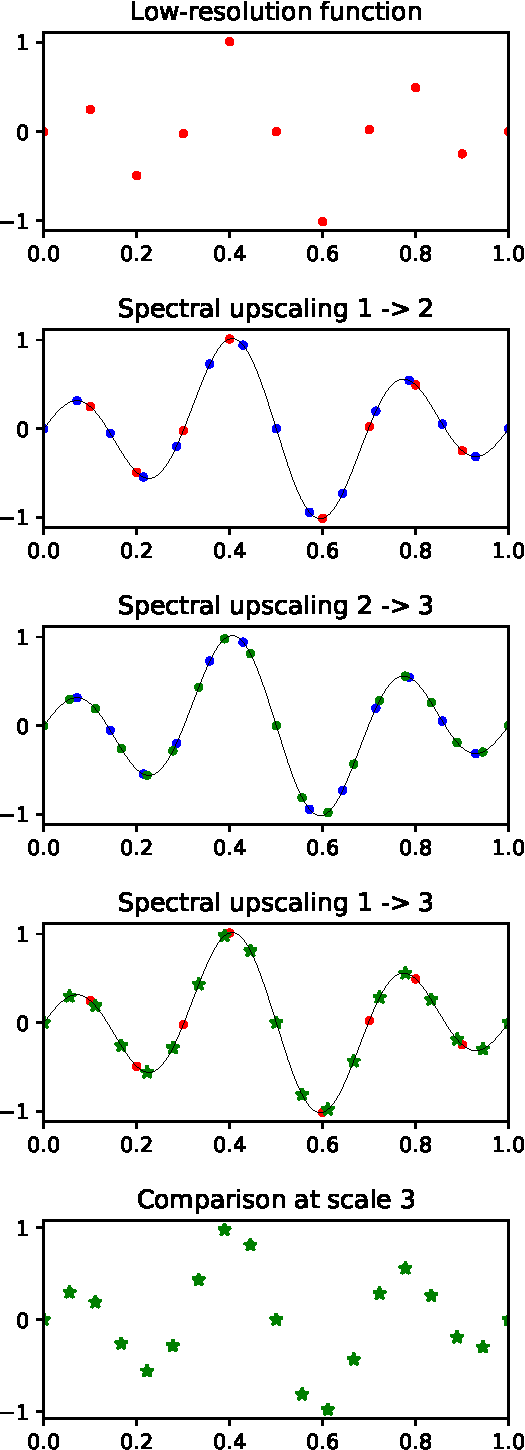
\includegraphics[width=0.38\textwidth]{interpolation_comparison_sp.pdf}
\end{center}
\caption{\label{fig:sp} Transitivity upscaling for a spectral interpolator. Initial low resolution (red dots), intermediate resolution (blue dots) and high resolution interpolated from intermediate or low resolution (green dots and stars, respectively). The black lines indicate the continuous interpolation function. Successive grids are not colocated.}
\end{figure}

Usual grid-points interpolators like the (bi-)linear interpolator are not transitive in general, as illustrated in figure \ref{fig:lin}.

\begin{figure}[!h]
\begin{center}
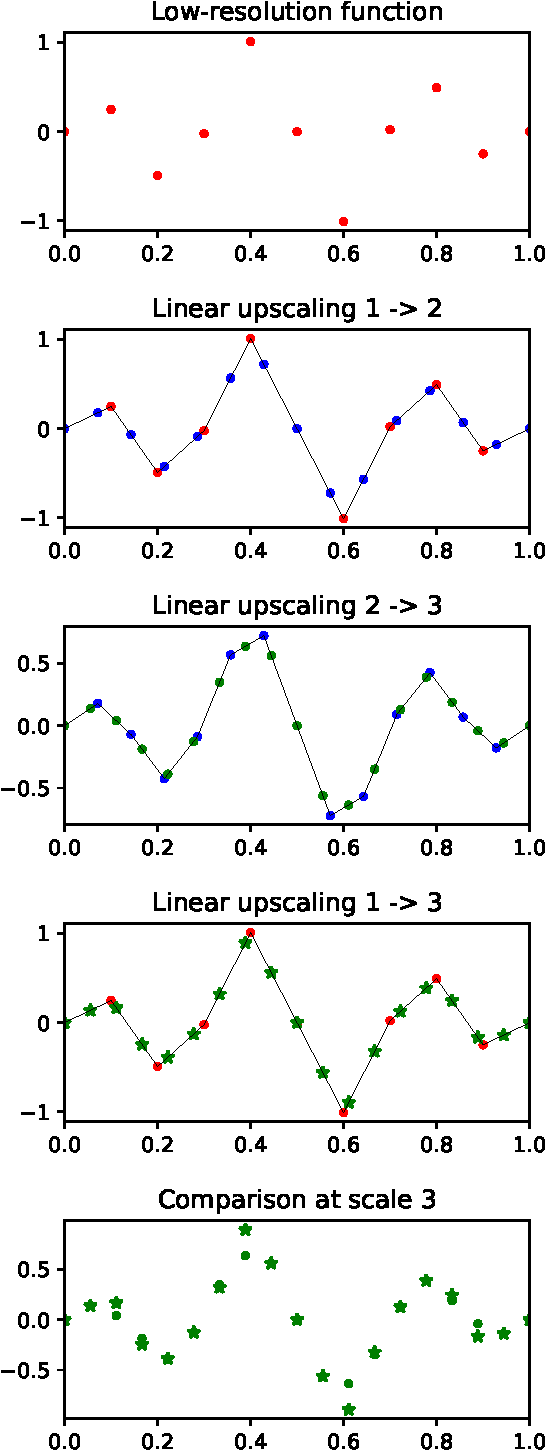
\includegraphics[width=0.39\textwidth]{interpolation_comparison_lin.pdf}
\end{center}
\caption{\label{fig:lin} Transitivity upscaling for a linear interpolator. Initial low resolution (red dots), intermediate resolution (blue dots) and high resolution interpolated from intermediate or low resolution (green dots and stars, respectively). The black lines indicate the continuous interpolation functions. Successive grids are not colocated.}
\end{figure}

\clearpage

An important exception is the (bi-)linear interpolator when coarse grid points are colocated with fine grid points, as shown in figure \ref{fig:lin_colocated}.

\begin{figure}[!h]
\begin{center}
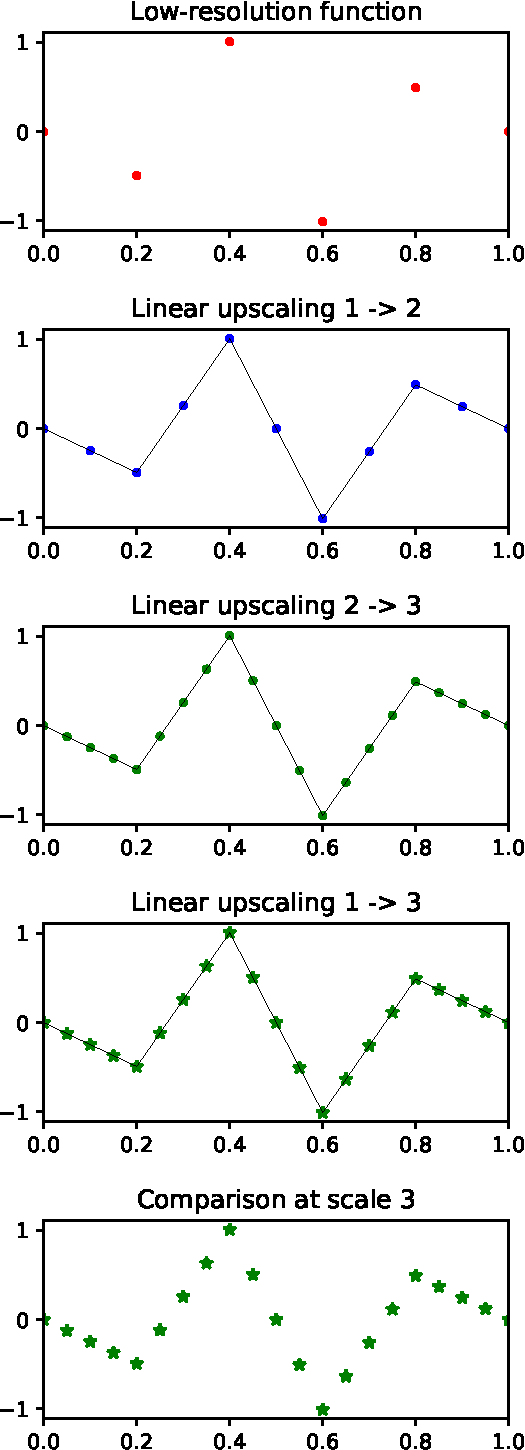
\includegraphics[width=0.39\textwidth]{interpolation_comparison_lin_colocated.pdf}
\end{center}
\caption{\label{fig:lin_colocated} Transitivity upscaling for a linear interpolator. Initial low resolution (red dots), intermediate resolution (blue dots) and high resolution interpolated from intermediate or low resolution (green dots and stars, respectively). The black lines indicate the continuous interpolation functions. Successive grids are colocated.}
\end{figure}

\clearpage

\subsection{Projective $\mathbf{B}$ family}
A vector $\boldsymbol{\gamma} \in \mathbb{R}^{n_K}$ of positive coefficients can define the diagonal matrices $\boldsymbol{\Gamma}_k \in \mathbb{R}^{n_k \times n_k}$:
\begin{align}
\Gamma_{k,\alpha \beta} = \left\{
\begin{array}{ccc}
\gamma_i & \text{ if } & \alpha = \beta \\
0 & \text{ if } & \alpha \ne \beta
\end{array}\right.
\end{align}
At resolution $\mathcal{R}_k$, the background error covariance matrix $\mathbf{B}_k$ is defined as:
\begin{align}
\mathbf{B}_k = \mathbf{S}_k \boldsymbol{\Gamma}_k \mathbf{S}_k^{-1}
\end{align}
A square-root $\mathbf{U}_k$ is simply:
\begin{align}
\mathbf{U}_k = \mathbf{S}_k \boldsymbol{\Gamma}_k^{1/2} \mathbf{G}_k
\end{align}
where $\mathbf{G}_k \in \mathbb{R}^{n_k \times m_k}$ can be any orthogonal matrix.\\
$  $\\
Thus:
\begin{align}
\mathbf{U}_k^\mathrm{T} \mathbf{T}^\mathbf{x}_{i \rightarrow k} & = \mathbf{G}^\mathrm{T}_k \boldsymbol{\Gamma}_k^{1/2} \mathbf{S}^\mathrm{T}_k \mathbf{S}_k \boldsymbol{\Delta}_{i \rightarrow k} \mathbf{S}^\mathrm{T}_i \nonumber \\
 & = \mathbf{G}^\mathrm{T}_k \boldsymbol{\Gamma}_k^{1/2}\boldsymbol{\Delta}_{i \rightarrow k} \mathbf{S}^\mathrm{T}_i
\end{align}
and
\begin{align}
\mathbf{T}^\mathbf{v}_{i \rightarrow k} \mathbf{U}_i^\mathrm{T} & = \mathbf{G}^\mathrm{T}_k \boldsymbol{\Delta}_{i \rightarrow k} \mathbf{G}_i \mathbf{G}^\mathrm{T}_i \boldsymbol{\Gamma}_i^{1/2} \mathbf{S}^\mathrm{T}_i \nonumber \\
& = \mathbf{G}^\mathrm{T}_k \boldsymbol{\Delta}_{i \rightarrow k}  \boldsymbol{\Gamma}_i^{1/2} \mathbf{S}^\mathrm{T}_i
\end{align}
Since $\boldsymbol{\Gamma}_k^{1/2}\boldsymbol{\Delta}_{i \rightarrow k} = \boldsymbol{\Delta}_{i \rightarrow k}  \boldsymbol{\Gamma}_i^{1/2}$, the projective $\mathbf{B}$ family condition \eqref{eq:projective_definition_U} is verified.

\end{document}

























\section{Full $\mathbf{B}$ preconditioning}

\subsection{Iterative solver}
A new variable $\delta \overline{\mathbf{x}}_k \in \mathbb{R}^n$ is defined as:
\begin{align}
\delta \overline{\mathbf{x}}_k = \mathbf{B}_k^{-1} \delta \mathbf{x}_k \ \Leftrightarrow \ \delta \mathbf{x}_k = \mathbf{B}_k \delta \overline{\mathbf{x}}_k
\end{align}
Linear system \eqref{eq:inc} is transformed into:
\begin{align}
\label{eq:inc_B}
\boxed{\mathbf{A}^{\overline{\mathbf{x}}}_k \delta \overline{\mathbf{x}}^a_k = \mathbf{b}^{\overline{\mathbf{x}}}_k}
\end{align}
with $\mathbf{A}^{\overline{\mathbf{x}}}_k \in \mathbb{R}^{n \times n}$ and $\mathbf{b}^{\overline{\mathbf{x}}}_k \in \mathbb{R}^{n}$ defined as:
\begin{align}
\mathbf{A}^{\overline{\mathbf{x}}}_k & = \mathbf{I}_n + \mathbf{H}_k^\mathrm{T} \mathbf{R}^{-1} \mathbf{H}_k \mathbf{B}_k \\
\mathbf{b}^{\overline{\mathbf{x}}}_k & =  \delta \overline{\mathbf{x}}^b_k + \mathbf{H}_k^\mathrm{T} \mathbf{R}^{-1} \mathbf{d}_k
\end{align}

The PLanczosIF method with a preconditioner $\mathbf{P}_k = \mathbf{B}\mathbf{C}_k$, where $\mathbf{C}_k \in \mathbb{R}^{n \times n}$ and $\mathbf{P}_k \in \mathbb{R}^{n \times n}$ is detailed in algorithm \ref{algo:planczosif}.\\

A common (but not unique) way to define the preconditioner $\mathbf{P}_k = \mathbf{B}\mathbf{C}_k$ consists in using the spectral Limited Memory Preconditioner (LMP) approximated from the Ritz pairs:
\begin{itemize}
\item For the first outer iteration ($k=1$): $\mathbf{C}_1 = \mathbf{I}_n$.
\item For subsequent outer iteration ($k>1$):
\begin{align}
\mathbf{C}_{k+1} = \mathbf{C}_k + \overline{\mathbf{V}}_k \left(\mathbf{\Lambda}_k^{-1} - \mathbf{I}_{I_k}\right) \mathbf{V}_k^\mathrm{T}
\end{align}
where
\begin{align}
\overline{\mathbf{V}}_k & = \mathbf{C}_k \underline{\overline{\mathbf{V}}}_k \\
\mathbf{V}_k & = \mathbf{B} \overline{\mathbf{V}}_k
\end{align}
\end{itemize}
It should be noted that the Ritz vectors are orthogonal with respect to the $\mathbf{P}_k$-inner product:
\begin{align}
\underline{\overline{\mathbf{V}}}_k^\mathrm{T} \mathbf{P}_k \underline{\overline{\mathbf{V}}}_k = \mathbf{I}_{I_k}
\end{align}
As a consequence, the inverse of $\mathbf{C}_{k+1}$ can be easily computed from the Woodbury matrix identity:
\begin{align}
\mathbf{C}_{k+1}^{-1} & = \mathbf{C}_k^{-1} - \mathbf{C}_k^{-1} \overline{\mathbf{V}}_k \left(\left(\mathbf{\Lambda}_k^{-1} - \mathbf{I}_{I_k}\right)^{-1}+\mathbf{V}_k^\mathrm{T} \mathbf{C}_k^{-1} \overline{\mathbf{V}}_k\right)^{-1} \mathbf{V}_k^\mathrm{T} \mathbf{C}_k^{-1} \nonumber \\
& = \left(\mathbf{I}_n-\underline{\overline{\mathbf{V}}}_k \left(\left(\mathbf{\Lambda}_k^{-1} - \mathbf{I}_{I_k}\right)^{-1}+\mathbf{I}_{I_k}\right)^{-1} \mathbf{V}_k^\mathrm{T}\right)\mathbf{C}_k^{-1} \nonumber \\
& = \left(\mathbf{I}_n+\underline{\overline{\mathbf{V}}}_k \left(\mathbf{\Lambda}_k-\mathbf{I}_{I_k}\right) \mathbf{V}_k^\mathrm{T}\right)\mathbf{C}_k^{-1}
\end{align}

\begin{algorithm}[!ht]
\caption{PLanczosIF algorithm with a preconditioner $\mathbf{P}_k = \mathbf{B}\mathbf{C}_k$\label{algo:planczosif}}
\begin{algorithmic}
\STATE Set the number of iterations: $I_k$
\STATE $  $
\STATE Objects sizes:
\STATE $\alpha_i$, $\beta_i \in \mathbb{R}$ for $0 \le i \le I_k$
\STATE $\mathbf{q}_i$, $\mathbf{r}_i$, $\overline{\mathbf{t}}_i$, $\mathbf{t}_i$, $\mathbf{v}_i$, $\mathbf{w}_i$, $\overline{\mathbf{z}}_i$, $\mathbf{z}_i \in \mathbb{R}^n$ for $0 \le i \le I_k$
\STATE $\mathbf{e_1} = [1,0,\dots,0]^\mathrm{T} \in \mathbb{R}^{I_k}$
\STATE $\mathbf{T}$, $\boldsymbol{\Theta}$, $\mathbf{Y}$, $\boldsymbol{\Lambda}_k \in \mathbb{R}^{I_k \times I_k}$
\STATE $\underline{\mathbf{V}}$, $\underline{\overline{\mathbf{V}}}_k \in \mathbb{R}^{n \times I_k}$
\STATE $  $
\STATE Initialization:
\STATE $\mathbf{v}_0 = 0$
\STATE $\mathbf{r}_0 = \delta \overline{\mathbf{x}}^b_k + \mathbf{H}_k^\mathrm{T} \mathbf{R}^{-1} \mathbf{d}_k$
\STATE $\overline{\mathbf{t}}_0 = \mathbf{C}_k \mathbf{r}_0$
\STATE $\mathbf{t}_0 = \mathbf{B} \overline{\mathbf{t}}_0$
\STATE $\beta_0 = \sqrt{\mathbf{r}_0^\mathrm{T} \mathbf{t}_0}$
\STATE $\mathbf{v}_1 = \mathbf{r}_0/\beta_0$
\STATE $\overline{\mathbf{z}}_1 = \overline{\mathbf{t}}_0/\beta_0$
\STATE $\mathbf{z}_1 = \mathbf{t}_0/\beta_0$
\STATE $\beta_1 = 0$
\STATE $  $
\FOR{$1 \le i \le I_k$}
\STATE Store the Lanczos vector $\mathbf{v}_i$ as the $i^\text{th}$ column of $\underline{\mathbf{V}}$
\STATE Update scalars and vectors:
\STATE $\mathbf{q}_i = \overline{\mathbf{z}}_i + \mathbf{H}_k^\mathrm{T} \mathbf{R}^{-1} \mathbf{H}_k \mathbf{z}_i - \beta_i \mathbf{v}_{i-1}$
\STATE $\alpha_i = \mathbf{q}_i^\mathrm{T} \mathbf{z}_i$
\STATE $\mathbf{w}_i = \mathbf{q}_i - \alpha_i \mathbf{v}_i$
\STATE $\overline{\mathbf{t}}_i = \mathbf{C}_k \mathbf{w}_i$
\STATE $\mathbf{t}_i = \mathbf{B} \overline{\mathbf{t}_i}$
\STATE $\beta_{i+1} = \sqrt{\mathbf{w}_i \mathbf{z}_i}$
\STATE $\mathbf{v}_{i+1} = \mathbf{w}_i/\beta_{i+1}$
\STATE $\overline{\mathbf{z}}_{i+1} = \overline{\mathbf{t}}_i/\beta_{i+1}$
\STATE $\mathbf{z}_{i+1} = \mathbf{t}_i/\beta_{i+1}$
\STATE Fill the tridiagonal matrix $\mathbf{T}$:
\STATE $T_{ii} = \alpha_i$
\IF{$i>1$}
\STATE $T_{(i-1)i} = T_{i(i-1)} = \beta_i$
\ENDIF
\ENDFOR
\STATE Compute $\left(\boldsymbol{\Theta},\mathbf{Y}\right)$, the eigendecomposition of $\mathbf{T} = \mathbf{Y} \boldsymbol{\Theta} \mathbf{Y}^\mathrm{T}$
\STATE Compute the analysis increment: $\delta \mathbf{x}^a_k = \mathbf{P}_k \underline{\mathbf{V}} \mathbf{Y} \boldsymbol{\Theta}^{-1} \mathbf{Y}^\mathrm{T} \left(\beta_0 \mathbf{e}_1\right)$
\STATE Store the Ritz pairs $\left(\boldsymbol{\Lambda}_k,\underline{\overline{\mathbf{V}}}_k \right) = \left(\boldsymbol{\Theta},\underline{\mathbf{V}} \mathbf{Y}\right)$
\end{algorithmic}
\end{algorithm}

\FloatBarrier

\subsection{Equivalence condition for preconditioners}
Both approaches are equivalent if the preconditioners are linked via:
\begin{align}
\label{eq:eq_cond_1}
\mathbf{P}^{1/2}_k = \mathbf{Q}^{1/2}_k \mathbf{U}
\end{align}
which is verified for the spectral preconditioner approximated with the Ritz pairs. Figure \ref{fig:map} summarize the relationships between the different quantities.

\begin{figure}[!ht]
\begin{center}
\tikzstyle{field}=[draw,thin,rounded corners,inner sep=3pt]
\begin{tikzpicture}[auto,>=latex]
\node[field] (a) {$\underline{\widetilde{\mathbf{V}}}_k$};
\node[field,below of=a,node distance=2cm] (b) {$\delta \mathbf{v}_k, \widetilde{\mathbf{V}}_k$};
\node[field,below of=b,node distance=4cm,xshift=-5cm] (c) {$\delta \overline{\mathbf{x}}_k,\overline{\mathbf{V}}_k$};
\node[field,below of=b,node distance=4cm,xshift=5cm] (d) {$\delta \mathbf{x}_k,\mathbf{V}_k$};
\node[field,below of=c,node distance=2cm] (e) {$\underline{\overline{\mathbf{V}}}_k$};

\node[circle,draw,inner sep=1pt,above of=a,node distance=0.9cm,xshift=-0.9cm] (ortho_lanczos) {$\perp_{\mathbf{I}_{I_k}}$};
\node[circle,draw,inner sep=1pt,below of=e,node distance=0.9cm,xshift=-0.9cm] (ortho_planczosif) {$\perp_{\mathbf{P}_k}$};


\node[above of=c,node distance=1.8cm] (leftside) {};
\node[above of=d,node distance=1.8cm] (rightside) {};
\node[right of=c,node distance=1.6cm] (bottomsideleft) {};
\node[left of=d,node distance=1.8cm] (bottomsideright) {};
\node[above of=bottomsideleft,node distance=5.0cm] (topsideleft) {};
\node[above of=bottomsideright,node distance=5.0cm] (topsideright) {};
\node[below of=e,node distance=2.4cm,xshift=-0.5cm] (bottomlabel1) {\begin{tabular}{@{\hspace{0.07cm}}c@{\hspace{0.07cm}}}
Model \\
space
\end{tabular}};
\node[right of=bottomlabel1,node distance=5.8cm] (bottomlabel2) {\begin{tabular}{@{\hspace{0.07cm}}c@{\hspace{0.07cm}}}
Control \\
space
\end{tabular}};
\node[right of=bottomlabel1,node distance=10.6cm] (bottomlabel3) {\begin{tabular}{@{\hspace{0.07cm}}c@{\hspace{0.07cm}}}
Model \\
space
\end{tabular}};

\path[->,thick] ([xshift=-0.1cm]a.south) edge node[left] {$\mathbf{Q}^{1/2}_k$} ([xshift=-0.1cm]b.north);
\path[<-,thick] ([xshift=0.1cm]a.south) edge node[right] {$\left(\mathbf{Q}^{1/2}_k\right)^{-1}$} ([xshift=0.1cm]b.north);
\path[<-,thick,bend left=50] ([yshift=0.1cm]a.east) edge node[right,xshift=0.2cm] {$\left(\mathbf{P}^{1/2}_k\right)^{-1}$} ([xshift=0.1cm]d.north);
\path[->,thick,bend left=50] ([yshift=-0.1cm]a.east) edge node[left,xshift=0.4cm,yshift=-0.8cm] {$\mathbf{P}^{1/2}_k$} ([xshift=-0.1cm]d.north);
\path[->,thick] (b.east) edge node[right,yshift=0.2cm,xshift=-0.2cm] {$\mathbf{U}$} ([yshift=0.2cm]d.west);
\path[<-,thick] (b.west) edge node[left,yshift=0.2cm] {$\mathbf{U}^\mathrm{T}$} ([yshift=0.2cm]c.east);
\path[<-,thick] ([yshift=0.1cm]c.east) edge node[above] {$\mathbf{B}^{-1}$} ([yshift=0.1cm]d.west);
\path[->,thick] ([yshift=-0.1cm]c.east) edge node[below] {$\mathbf{B}$} ([yshift=-0.1cm]d.west);
\path[->,thick] ([xshift=0.1cm]c.south) edge node[right] {$\mathbf{C}^{-1}_k$} ([xshift=0.1cm]e.north);
\path[<-,thick] ([xshift=-0.1cm]c.south) edge node[left] {$\mathbf{C}_k$} ([xshift=-0.1cm]e.north);
\path[<-,thick,bend left=-30] ([yshift=0.1cm]e.east) edge node[above] {$\mathbf{P}_k^{-1}$} ([xshift=-0.12cm]d.south);
\path[->,thick,bend left=-30] ([yshift=-0.1cm]e.east) edge node[below] {$\mathbf{P}_k$} ([xshift=0.12cm]d.south);

\path[-,thick,dashed] ([xshift=-2cm]leftside.east) edge node[above] {Lanczos algorithm} ([xshift=2cm]rightside.west);
\path[-,thick,dashed] ([xshift=-2cm]leftside.east) edge node[below] {PLanczosIF algorithm} ([xshift=2cm]rightside.west);
\path[-,thick,dashed] ([yshift=-5cm]bottomsideleft.north) edge node {} ([yshift=2.7cm]topsideleft.south);
\path[-,thick,dashed] ([yshift=-5cm]bottomsideright.north) edge node {} ([yshift=2.7cm]topsideright.south);

\path[-,thick,bend left=-50] (a.north) edge node {} (ortho_lanczos.east);
\path[->,thick,bend left=-50] (ortho_lanczos.south) edge node {} (a.west);
\path[-,thick,bend left=-50] (e.west) edge node {} (ortho_planczosif.north);
\path[->,thick,bend left=-50] (ortho_planczosif.east) edge node {} (e.south);
\end{tikzpicture}
\end{center}
\caption{Map of spaces and links between them. Circles indicate orthogonality properties.}
\label{fig:map}
\end{figure}

\FloatBarrier





With the full $\mathbf{B}$ preconditioning, $\mathbf{B}^{-1}$ can be applied on both side of equation \eqref{eq:back_inc}:
\begin{align}
\label{eq:back_inc_B}
\boxed{\delta \overline{\mathbf{x}}^b_k = - \sum_{i=1}^{k-1} \delta \overline{\mathbf{x}}^a_i}
\end{align}
and with the square-root $\mathbf{B}$ preconditioning, 


\begin{align}
\delta \mathbf{x}^a_k = \mathbf{B}_k \delta \overline{\mathbf{x}}^a_k
\end{align}
or

\begin{align}
\label{eq:correct_dxb}
\delta \overline{\mathbf{x}}^b_k & = \mathbf{B}^{-1}_k \delta \mathbf{x}^b_k \nonumber \\
& = \mathbf{B}^{-1}_k \left(\mathbf{x}^b_k - \mathbf{x}^g_k\right) \nonumber \\
& = \mathbf{B}^{-1}_k \mathbf{T}^\mathbf{x}_{K \rightarrow k} \left(\mathbf{x}^b - \mathbf{x}^{g+}_k\right)
\end{align}
or

\begin{align}
\label{eq:back_inc_Bvar}
\boxed{\delta \overline{\mathbf{x}}^b_k = - \sum_{i=1}^{k-1} \mathbf{T}^\mathbf{x}_{i \rightarrow k} \delta \overline{\mathbf{x}}^a_i}
\end{align}
and

\begin{align}
\label{eq:consistent_B}
\delta \mathbf{x}^b_k & = \mathbf{B}_k \delta \overline{\mathbf{x}}^b_k
\end{align}
or



\section{Preconditionings equivalence}

When the resolution changes between outer iterations, the equivalence between full $\mathbf{B}$ and square-root $\mathbf{B}$ preconditionings is not guaranteed anymore. This section looks for equivalence conditions.

\subsection{Equivalence condition on the guess}
Two kinds of conditions can be required to get similar results with both preconditionings:
\begin{enumerate}
\item $\delta \mathbf{x}^{a+}_{k-1}$ has to be computed in a similar way for both preconditionings. This condition is sufficient for the theoretical method. It is not required for the consistent method, for which $\delta \mathbf{x}^{a+}_{k-1}$ is not required.
\item For the standard and consistent methods, equations \eqref{eq:back_inc_Bvar} and \eqref{eq:back_inc_Uvar} are related with:
\begin{align}
\mathbf{U}^\mathrm{T}_k \delta \overline{\mathbf{x}}^b_k & = \delta \mathbf{v}^b_k \nonumber \\
\Leftrightarrow \ - \mathbf{U}^\mathrm{T}_k  \sum_{i=1}^{k-1} \mathbf{T}^\mathbf{x}_{i \rightarrow k} \delta \overline{\mathbf{x}}^a_i & = - \sum_{i=1}^{k-1} \mathbf{T}^\mathbf{v}_{i \rightarrow k} \delta \mathbf{v}^a_i
\end{align}
If the previous outer iterations were equivalent for both preconditionings, then for $i \in [1,k-1, \delta \mathbf{v}^a_i = \mathbf{U}^\mathrm{T}_i \delta \overline{\mathbf{x}}^a_i$ so this condition becomes:
\begin{align}
\mathbf{U}^\mathrm{T}_k \mathbf{T}^\mathbf{x}_{i \rightarrow k} = \mathbf{T}^\mathbf{v}_{i \rightarrow k} \mathbf{U}^\mathrm{T}_i
\end{align}
which is the same as the condition \eqref{eq:projective_definition_U} for a projective $\mathbf{B}$ family.
\end{enumerate}

\subsection{Equivalence condition on Ritz vectors}
If the resolution changes, the equivalence condition for preconditioners \eqref{eq:eq_cond_1} must be adapted since $\mathbf{U}$ depends on $k$:
\begin{align}
\mathbf{P}^{1/2}_k = \mathbf{Q}^{1/2}_k \mathbf{U}_k
\end{align}
In the case where the preconditioners are built using Ritz vectors, the map of Figure \ref{fig:map} shows that this condition is equivalent to a relation between the Ritz vectors:
\begin{align}
\mathbf{W}_k\underline{\overline{\mathbf{V}}}_k = \underline{\widetilde{\mathbf{V}}}_k
\end{align}
with $\mathbf{W}_k = \left(\mathbf{Q}^{1/2}_k\right)^{-1} \mathbf{U}^\mathrm{T}_k \mathbf{C}_k$.\\

If the resolution changes, the Ritz vectors also require an interpolation from their original resolution to the resolution $\mathcal{R}_k$ in order to build the preconditioner for iteration $k$, so the condition becomes:
\begin{align}
\mathbf{W}_k \mathbf{T}^\mathbf{x}_{i \rightarrow k} \underline{\overline{\mathbf{V}}}_i = \mathbf{T}^\mathbf{v}_{i \rightarrow k} \underline{\widetilde{\mathbf{V}}}_i
\end{align}
which is verified if and only if:
\begin{align}
\label{eq:eq_cond_3}
\mathbf{W}_k \mathbf{T}^\mathbf{x}_{i \rightarrow k} = \mathbf{T}^\mathbf{v}_{i \rightarrow k} \mathbf{W}_i
\end{align}
A last set of conditions regarding the orthogonality of Ritz vectors, which should not be lost during the interpolation process, should be verified:
\begin{align}
\label{eq:eq_cond_4}
\left(\mathbf{T}^\mathbf{x}_{i \rightarrow k} \underline{\overline{\mathbf{V}}}_i\right)^\mathrm{T} \mathbf{P}_k\left(\mathbf{T}^\mathbf{x}_{i \rightarrow k} \underline{\overline{\mathbf{V}}}_i\right) = \mathbf{I}_{I_k}
\end{align}
and
\begin{align}
\label{eq:eq_cond_5}
\left(\mathbf{T}^\mathbf{v}_{i \rightarrow k} \underline{\widetilde{\mathbf{V}}}_i\right)^\mathrm{T} \left(\mathbf{T}^\mathbf{v}_{i \rightarrow k} \underline{\widetilde{\mathbf{V}}}_i\right) = \mathbf{I}_{I_k}
\end{align}

\section{Equivalence overview}
This section gives an overview of equivalences between methods and preconditioning. It focuses on the guess conditions, and assumes that Ritz vectors are not used. In the following arrays, a green checkmark \textcolor{green}{\cmark} indicates that results are similar, and a red cross \textcolor{red}{\xmark} indicates that results are different. Obviously, all methods and preconditionings give the same results for the first outer iteration, so the equivalence arrays are shown for $k>1$ only. For the theoretical and standard methods, we can use either the complete expressions of equations \eqref{eq:transitive_condition_B}-\eqref{eq:transitive_condition_U} or the simplified expressions of equations \eqref{eq:projective_condition_B}-\eqref{eq:projective_condition_U} to compute $\delta \mathbf{x}^{a+}_{k-1}$.
